%%%%%%%%%%%%%%%%%%%%%%%%%%%%%%%%%%%%%%%%%%%%%%%%%%%%%%%
% A template for Wiley article submissions.
% Developed by Overleaf. 
%
% Please note that whilst this template provides a 
% preview of the typeset manuscript for submission, it 
% will not necessarily be the final publication layout.
%
% Usage notes:
% The "blind" option will make anonymous all author, affiliation, correspondence and funding information.
% Use "num-refs" option for numerical citation and references style.
% Use "alpha-refs" option for author-year citation and references style.

%\documentclass[num-refs]{wiley-article}
%\documentclass[alpha-refs]{wiley-article}
%\documentclass[10pt]{elsarticle}
\documentclass{IEEEtran}
% Add additional packages here if required

\usepackage{siunitx}
\usepackage[font=footnotesize, justification = centering]{caption}
\usepackage[font=footnotesize]{subcaption}
\usepackage{amsmath}
\usepackage[ruled,vlined]{algorithm2e} %for writing pseudocodes
\usepackage{graphicx}
% Update article type if known
%\papertype{Research Article}
% Include section in journal if known, otherwise delete


\title{Static and Dynamic Controller Assignment Algorithms for Software Defined Networks}

% List abbreviations here, if any. Please note that it is preferred that abbreviations be defined at the first instance they appear in the text, rather than creating an abbreviations list.
%\abbrevs{ABC, a black cat; DEF, doesn't ever fret; GHI, goes home immediately.}

% Include full author names and degrees, when required by the journal.
% Use the \authfn to add symbols for additional footnotes and present addresses, if any. Usually start with 1 for notes about author contributions; then continuing with 2 etc if any author has a different present address.
%\author[1]{Talha Ibn Aziz}
%\author[1]{Shadman Protik}
%\author[1]{Md Sakhawat Hossen}
%\author[2]{Salimur Choudhury}
%\author[1]{Muhammad Mahbub Alam}

%\contrib[\authfn{1}]{Equally contributing authors.}

% Include full affiliation details for all authors

%\affil[1]{Department of Computer Science and Engineering, %Islamic University of Technology, Dhaka, Bangladesh}
%\affil[2]{Department of Computer Science, Lakehead University, %Thunder Bay, Ontario, Canada}

%\corraddress{Salimur Choudhury, Department of Computer %Science, Lakehead University, Thunder Bay, Ontario, Canada}
%\corremail{salimur.choudhury@lakeheadu.ca}

% Include the name of the author that should appear in the running header
%\runningauthor{Talha et al.}

\pagenumbering{gobble}

\setlength{\textfloatsep}{10pt plus 1.0pt minus 2.0pt}



\author{\IEEEauthorblockN{Talha Ibn Aziz\IEEEauthorrefmark{1}}
	
	\IEEEauthorblockA{\IEEEauthorrefmark{1}Department of Computer Science and Engineering, Islamic University of Technology, Dhaka, Bangladesh} \\
	Email:  \IEEEauthorrefmark{1}talhaibnaziz@iut-dhaka.edu
}

\begin{document}
	
	\maketitle
	
	
	
	\begin{abstract}
		
		\noindent 
		Summarize the paper.
		
		\begin{IEEEkeywords}
			
		\end{IEEEkeywords}
		
	\end{abstract}
	
	
	
	\section{Introduction}
	Software Defined Networks (SDNs) simplifies network management by decoupling the traditional protocol stack in data and control planes, which consist of switches and controllers, respectively. The controllers replace the switches as the decision taking entities of the SDNs and the switches only retain their data-forwarding capabilities, which simplifies switch designs and configurations. Due to scalability and reliability issues \cite{scalability2013dixit, scalability2013yeganeh} paired with the formation of bottle-necks in moderate-sized networks, the initial design of a single controller \cite{greene2009tr10} is replaced by a multiple-controller architecture. The resultant problem is well-known as the NP-Hard Controller Placement Problem (CPP) which deals with placing an optimal number of controllers to improve network throughput \cite{cppsurvey2017, cppsurvey2018, sdnsurvey2017}. The multiple constraints that need satisfying include minimizing network latencies, deployment costs, energy consumption and maximizing reliability and resilience. Researches in recent years propose several approximations which deal with one or more of these constraints. 
	
	\begin{itemize}
		\item SDN to CPP (multiple controllers)
		\item Latency and Load Balancing
		\item Our Contributions and have to define flow setup latency
	\end{itemize}

	\section{Background and Related Works}
	Literature Review of Latency Based Solutions and Load Balancing.
		
	\section{System Model}
	The latency or delay of sending a data packet from source to destination consists of four components namely propagation latency, transmission latency, processing latency and queuing latency \cite{forouzan2006data}. Overall decrease in latency results in a network with high throughput and efficiency. In traditional networks, propagation latency latency is negligible as data signals propagate at nearly the speed of light. Queuing latency is the time a packet waits in the buffer or queue, processing latency is the time required to match a packet with routing tables and the time required for converting the entire data packet into signals is transmission latency. In Software-Defined Networks, the flow-setup latency can be included into the processing latency.
	
	The networks \cite{knight2011internet} are represented as a bi-directional graph $G=(S,L)$, where, $S$ represents the set of switches and $L$ represents the set of edges or links between the switches. The link weights are bandwidths
	
	\begin{itemize}
		\item Network - breakdown into different latencies and find which we focus on and why.	
		\item Load of switches and controllers and our assumptions
		\item mention interchangeable terms: network and graph, node and switch, link and edge, sub-network and cluster, distance and latency
		\item mention what edge weight represents (bandwidth to latency/distance)
	\end{itemize}
	
	
	\section{Proposed Method}
	
	My proposed method consists of three algorithms - Latency Based Clustering (LBC), Controller Selection Algorithm (CSA) and Best-first-search Load Balancing (BLB). LBC clusters the network into a given number of sub-networks ($k$) and CSA places a controller in each sub-network, resulting in a static controller-switch assignment. BLB is a dynamic load balancing algorithm which periodically reassigns switches to avoid over-burdening a controller. The above mentioned algorithms are explained in detail in sections \ref{lbc}, \ref{csa} and \ref{blb}, respectively.
	
	\subsection{Latency Based Clustering (LBC)} \label{lbc}
	
	%Explain what our previous work did and what are its shortcomings
	My previous work Degree-based Balanced Clustering (DBC) \cite{aziz2019degree} selects the nodes with the highest degrees in an unweighted network as cluster heads to facilitate better communication. Ensuring that the cluster heads are a minimum distance ($T_d$) apart from each other, DBC then places controllers based on inter-controller and intra-controller distances. However, the controllers are rarely in the same positions as the cluster heads, invalidating the degree-based cluster head selection. We propose a novel clustering algorithm LBC, which selects cluster-centers instead of cluster-heads. These cluster centers are the foundations of the clusters and they ensure that the clusters are evenly distributed throughout the network instead of being centralized at a certain region.
	
	The controller of a network needs to frequently communicate with switches and other controllers (for multiple controllers). Accordingly, assuming that the network is small enough to be managed by one controller, it should be placed at the center. According to graph theory, the center of a graph has the property of being nearest to all the other vertices \cite{wilson1979introduction} and can be selected by minimizing the average or maximum distance of a node from the remaining nodes, which can be calculated as follows:
	
	\begin{equation} \label{eqn:maxDis}
		maxDis_{s\in S} = max_{d\in S}(dis(s,d))
	\end{equation}
	\begin{equation} \label{eqn:avgDis}
		avgDis_{s \in S} = \frac{\sum_{d\in S}^{d\ne s}dis(s,d)}{|S|-1}
	\end{equation}
	
	\begin{figure}
		\centering
		\includegraphics[width=\linewidth]{Images/aarnet2009cc.png}
		\caption{Existing network of Australia (AARNET: collected in 2009, updated in 2011) showing the centers of the network.}
		\label{fig:aarnetcc}
	\end{figure}

	here, $maxDis_{s}$ and $avgDis_s$ are respectively the maximum and average distances from the source $s$ to any other destination node $d$ in the network $S$. The shortest path distance from $s$ to $d$ is denoted by $dis(s,d)$. The maximum distance or worst case latency (Equation \ref{eqn:maxDis}), when determines the center of the network, can vary greatly in the presence of distant and isolated nodes (Figure \ref{fig:aarnetcc}). Conversely, the average case latency (Equation \ref{eqn:avgDis}) is the better center-selection criterion of the two. Therefore, I select the node with the minimum average distance as the center of the network.
	
	Contrarily, for larger networks, when placing multiple controllers, multiple sub-networks must be formed which makes the center selection process troublesome. To ensure equal division of the network, the cluster-centers must be equally distant from each other and the clusters must expand from the centers. The selection of equidistant centers in a network is a well known classical NP-hard problem of computer science - \textit{The vertex k-center problem} \cite{kariv1979algorithmic}, which has many optimal approximations. My algorithm LBC (Algorithm \ref{algo:lbc}) utilizes the latencies between switches to provide a solution which divides the network optimally while ensuring that each cluster contains potential controller positions.
	
	\begin{algorithm}
		\SetAlgoLined
		\KwResult{Set of Cluster-Centers, $CC$ }
		$dis := all~possible~node~pair~shortest~distances$\;
		$sumDis_{s \in S} := \sum_{d \in S, d \ne s}dis(s,d)$\;
		$CC := \emptyset$, $k :=$ required number of controllers\;
		\While{$|CC| < k$}{
			$s_{cc}\in S$, where $sumDis_{s_{cc}} \le sumDis_{t\in S}$\;
			$CC := CC + s_{cc}$\; 
			Create a new cluster $S_i$, where $S_i := s_{cc} + \big(\frac{|S|}{k}-1\big)~nearest~neighbors~of~s_{cc}$ in terms of hop distance\;
			\ForEach{switch $s_i \in S_i$}{
				Subtract $dis(s_i, s)$ from $sumDis_s$ for all ${s \in S-S_i}$
			}
			$S = S - S_i$
		}
		\caption{Latency Based Clustering (LBC)} \label{algo:lbc}
	\end{algorithm}

	In an ideal scenario, I deduce that, for a network to be divided into $k$ clusters, each cluster should have $\frac{|S|}{k}$ switches. Therefore, every two cluster-center must have enough distance in between them to accommodate at least $\frac{|S|}{k}$ switches, which can be considered the \textit{ideal cluster-size}. I use the cumulative distance of a node $sumDis_s = avgDis_s \times (|S|-1)$, which is proportional to its average distance, paired with the ideal cluster-size to determine the cluster-centers. The cumulative distance is lowest at the center, increasing gradually towards the periphery of the network. In each iteration, I select the node with the least cumulative as a cluster-center, expand hop by hop from there until I have an ideal cluster-size. Consequently, I remove the selected nodes from the network and subtract their distances from the cumulative of all the other nodes and the process resets itself. Ultimately, in each iteration, I are determining the center of a theoretically-new network until I have $k$ cluster-centers. The process of cluster-center selection is similar for all values of $k$, except for $k=2$, in which case I select the nodes with minimum average distances. Excluding the node removal results in an equally divided network as cluster-center grouping is not a problem for a small value of $k$.

	\subsection{Controller Selection Algorithm (CSA)} \label{csa}
	
	The algorithm LBC provides a list of cluster-centers which are the starting points for each sub-network. The Controller Selection Algorithm (CSA) creates clusters once more from these cluster-centers to avoid formation of overlapping clusters or isolated cluster-centers, and then selects a controller position for each cluster. The nodes are included in the clusters of the nearest clusters-centers in terms of shortest path distance $dis(i,j)_{i,j \in S}$, which ends the cluster formation process.
	
	
	\begin{algorithm}
		\SetAlgoLined
		\KwResult{Set of Controllers, $C$ }
		$dis := all~possible~node~pair~shortest~distances$\;
		$CC_{i=1}^k :=$ \textbf{LBC}~Cluster~Centers\;
		$S_{i=1}^k := k~empty~Clusters$\;
		$\phi_{s\in S}(s) :=$ intra-cluster latencies\;
		$\sigma_{s\in S}(s) :=$ inter-cluster latencies\;
		\For{center $s_{i} \in CC$}{
			$S_i$ = $S_i + s_{cc}$;
		}
		\ForEach{switch $s \in S$}{
			\If{$s \not \in CC$}{
				$s_{cc}=\min(dis(s,s_i)_{s_i \in CC})$\;
				Include $s$ in cluster of $s_{cc}$;
			}
		}
		\ForEach{switch $s \in S$}{
			$S_i :=$ cluster of $s$\;
			$\phi(s)=\sum_{t\in S_i} dis(s,t)$\;
			$\sigma(s)=\sum_{t\in (S-S_i)} dis(s,t)$\;
		}
		\ForEach{cluster $S_i \subset S$}{
			$s_c:=\min(\phi(s_i)\times \alpha + \sigma(s_i)\times(1-\alpha))$ for all $s_i \in S_i$\;
			$C:=C+s_c$\;
		}
		\caption{Controller Selection Algorithm (CSA)} \label{algo:csa}
	\end{algorithm}
	
	The controller positions must have better connectivity with the switches and controllers compared to the other nodes. However, both controller-to-controller and controller-to-switch distances cannot be minimized simultaneously. Furthermore, distance from a controller to any other node or controller cannot be calculated without placing a controller first, which results in a paradoxical scenario. Therefore, I utilize the controller selection method of our previous work \cite{aziz2019degree}, which calculates both inter-cluster ($\sigma$) and intra-cluster ($\phi$) distances as a replacement of inter-controller and intra-controller distances, respectively. I also introduce a new constant ($\alpha$) to provide an option to control their priority when selecting controller positions. Finally, the controller position ($C_i$) for a cluster $S_i$, is calculated as follows:
	
	\begin{equation} \label{eqn:intra}
		\phi(s)_{s\in S_i} = \frac{1}{|S_i|-1}\sum_{u\in S_i} dis(s,u)
	\end{equation}
	
	\begin{equation} \label{eqn:inter}
		\sigma(s)_{s\in S_i} = \frac{1}{|S-S_i|}\sum_{v\in (S-S_i)} dis(s,v)
	\end{equation}
	
	\begin{equation} \label{eqn:totlat}
		C_i = \min(\phi(s)\times \alpha + \sigma(s)\times(1-\alpha))
	\end{equation}
	
	here, $\alpha$ is the normalized constant which controls the effect of $\sigma(s)$ and $\phi(s)$, $s$ is any node in cluster $S_i$, and $C_i$ is its selected controller position.
	
	The highest possible value of $\alpha$ is $1$, which nullifies the effect of $\sigma$ and selects controllers considering only intra-cluster distances. Meanwhile, for $\alpha = 0$, controllers are placed solely considering inter-cluster distances. The value of $\alpha$ can be changed to better suit the requirement of the network administrator. I call the modified controller selection criterion which is a combination of the intra-cluster and inter-cluster distances, the \textit{inverse priority}. The node with the least possible \textit{inverse priority} in a sub-network is selected as its controller position. The pseudo-code of the Controller Selection Algorithm is given below in Algorithm \ref{algo:csa}.
	

	\subsection{Best-first-search Load Balancing (BLB)} \label{blb}
	
	For a fixed controller-switch assignment scheme ($S\rightarrow C$), the loads of the controllers vary due to changing loads of the switches. However, once a controller is placed, changing its position is both costly and inefficient. To balance the constantly changing loads of the controllers, we propose a dynamic load balancing algorithm BLB (Algorithm \ref{algo:blb}). BLB considers each controller-switch assignment scheme as a separate network state and the target is to reach the optimal state, where the load of the network is balanced.
	
	\begin{algorithm}
		\SetAlgoLined
		\KwResult{Assignment of Switches, $S \rightarrow C$ }
		$S_{i=1}^k := $ \textbf{CSA} Clusters\;
		$state := S \rightarrow C$, current assignment of switches\;
		Set of all possible new states, $Pstates := {state}$\;
		\While{$Pstates \ne \emptyset$}{
			$state := \min(\varepsilon(Pstates))$\;
			$Pstates := \emptyset$\;
			\ForEach{border switch $s\in S$}{
				New assignments $Nstate := state$\;
				Change assignment of switch $s$ to controller of adjacent cluster in $Nstate$\;
				\If{$\varepsilon(Nstate)<\varepsilon(state)$}{
					$Pstates := Pstates + Nstate$\;
				}
			}
		}
		\caption{BestFS Load Balancing (BLB)} \label{algo:blb}
	\end{algorithm}
	
	I assume that each controller has identical processing capacity and the switches have varying loads and denote the loads of the switches as $l_1, l_2, . .$ and so on. The total load of the network $S$, at any state can be calculated as,
	
	\begin{equation}
		L=\sum_{i=1}^{|S|}l_i
	\end{equation}
	
	Therefore, ideally, the load of a controller in the target state should be $\frac{L}{k}$, where $k$ is the number of controllers. However, when switches are assigned to distant controllers to maintain an ideal load distribution, excess traffic may be generated (Figure yet to be attached). The extra traffic contributes to and overall increase in latency and decrease in network throughput. To avoid such overlapping of clusters, I prioritize distance over load balancing, and express the problem as a Heuristic (Informed) Search with the following foundations:
	
	\subsubsection{Search Space and Root State}
	The entire search space is a graph where each node corresponds to a \textit{state}. A state is a valid controller-switch assignment scheme where there are multiple controllers and every switch is assigned to a single controller. The \textit{Root state} of the graph is the resultant assignment of switches when LBC and CSA are applied on a network.
	
	\subsubsection{Child State}
	All the children of any node of the search space graph must be valid \textit{states}. Any \textit{Child state} is similar to its parent state except one switch, which is at the border of any cluster and is reassigned to the controller of the adjacent cluster. All such combinations constitute the set of Child states of any parent state.
	
	\subsubsection{Error Function}
	The error function $\varepsilon$ determines the acceptability of the current \textit{state} and is calculated as follows:
	\begin{equation}
		\varepsilon(state) = \sum_{i=1}^{k}\Big(L_i - \frac{L}{k}\Big)^2
	\end{equation}
	
	where, $L_i$ is the load of a controller, which is the cumulative load of the switches assigned to it. Squaring the differences give more priority to controllers whose loads are more imbalanced compared to others. Finally, halving the error nullifies the error value increase due to under-loaded controllers.
	
	\subsubsection{Heuristic}
	A greedy heuristic is disadvantageous as it provides a sub-optimal solution. However, as my goal is not an absolute and optimal solution, rather a local optima where no clusters are overlapping, I select the error function as the heuristic. I use the Best First Search (BFS) technique with pruning to solve this problem, which selects the child state with the least error as the new assignment scheme in each iteration. When there is no child state with less error compared to the Root state (Figure \ref{fig:aarnet2009l1}), the child states are pruned to minimize computational complexity. Conversely, all the child states with equal or more error are pruned at each iteration and the algorithm continues until the target state or a controller-switch assignment scheme with minimum error is achieved  (Figure \ref{fig:aarnet2009l2}).
	
	\onecolumn
	
	\begin{figure}
		\centering
		\begin{subfigure}{0.35\textwidth}
			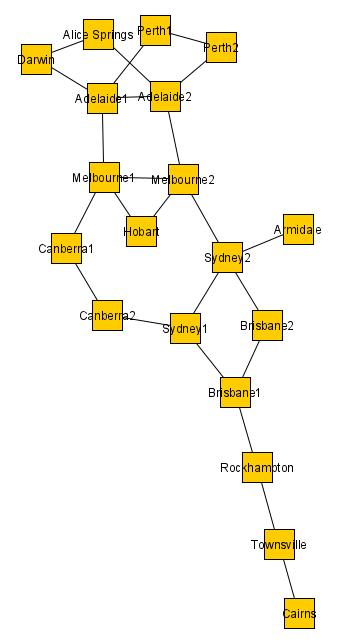
\includegraphics[width=\linewidth]{Images/Aarnet.jpg}
			\caption{Original Aarnet Network (rearranged)}
			\label{fig:aarnet2009}
		\end{subfigure}
		~
		\begin{subfigure}{0.35\textwidth}
			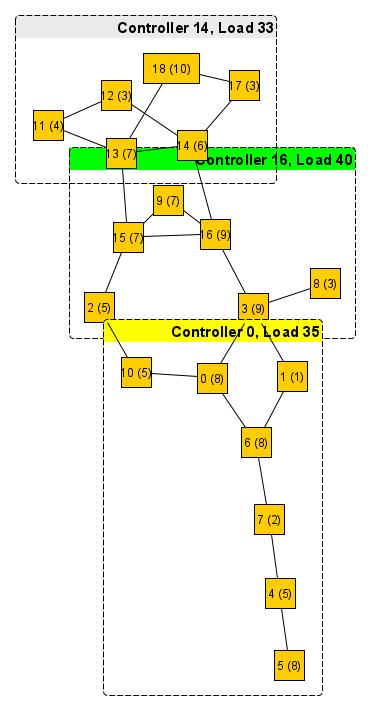
\includegraphics[width=\linewidth]{Images/Aarnet_Load_1.jpg}
			\caption{Root state with no child state}
			\label{fig:aarnet2009l1}
		\end{subfigure}
		~
		\begin{subfigure}{0.9\textwidth}
			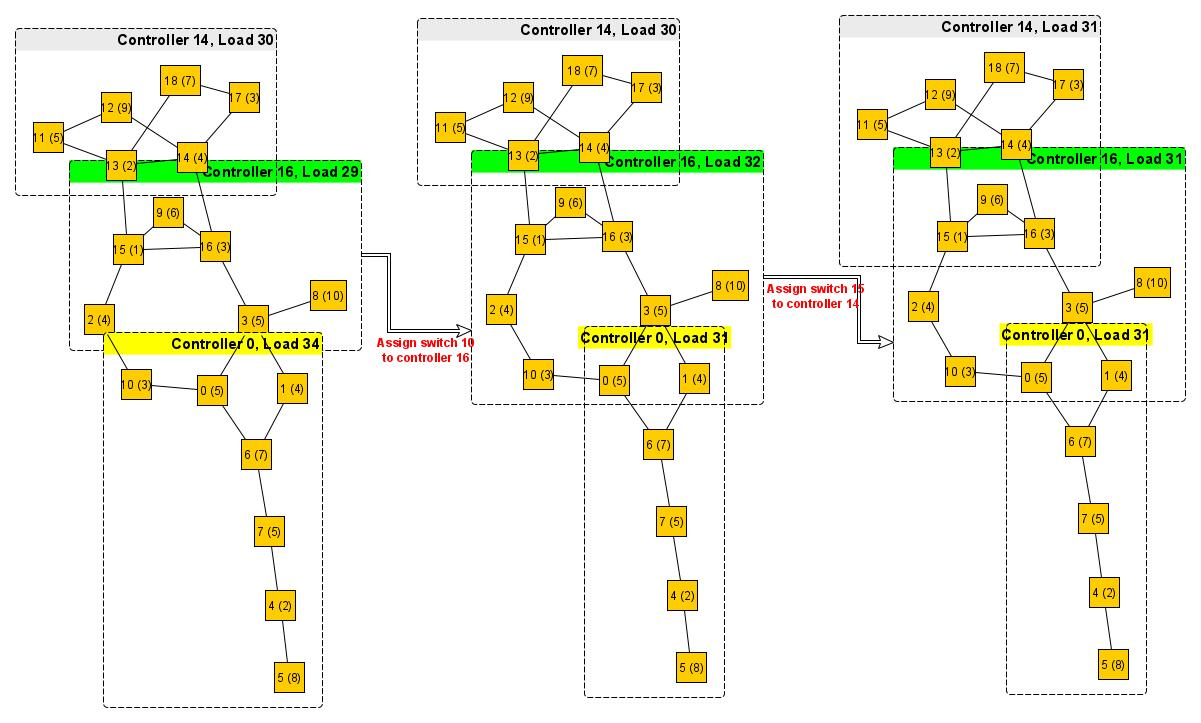
\includegraphics[width=\linewidth]{Images/Aarnet_Load_2.jpg}
			\caption{Optimal assignment scheme achieved after three iterations}
			\label{fig:aarnet2009l2}
		\end{subfigure}
		\caption{The BLB algorithm applied on Aarnet Network variations with randomized loads. Each switch is represented by a switch id, followed by its load. Each cluster has its own controller position and load marked above.}
	\end{figure}
	
	\twocolumn
	\section{Performance Evaluation}
	
	\subsection{Simulation Environment}
	I create a simulation environment which uses a high-level language C++, to perform experiments on existing network topologies collected from the Internet Topology Zoo \cite{knight2011internet}. The Topology Zoo contains a total of 261 existing network topologies, out of which 18 networks have islands (isolated nodes). Therefore, I perform my experiments on the remaining networks. A summary of our experimental networks are given in Table \ref{tab:zooSummary}.
	\begin{table}
		\centering
		\caption{A summary of our Experimental Networks} \label{tab:zooSummary}
		\begin{tabular}{|l|c|}
			\hline
			\textbf{Category} & \textbf{Data} \\
			\hline
			Total number of networks & 243 \\
			\hline
			Number of unweighted networks & 134 \\
			\hline
			Maximum number of nodes & 754 \\
			\hline
			Minimum number of nodes & 4 \\
			\hline
			Networks with multi-edges & 82\\
			\hline
			Average Edge per Node & 1.285 \\
			\hline
		\end{tabular}
	\end{table}
	The weights of the links in weighted networks are their bandwidths in \textit{Gbps} (Giga-bits per second). I convert the link bandwidth into latencies (milliseconds), assuming each data packet is of standard size (1500 bytes). The maximum bandwidth is considered for links with variable bandwidths and all fiber-optic cables without available bandwidth information are assumed to have 1 Gbps bandwidths. I consider networks with identical edge weights as unweighted.
	\subsection{Performance Metrics}
	
	\begin{figure}
		\centering
		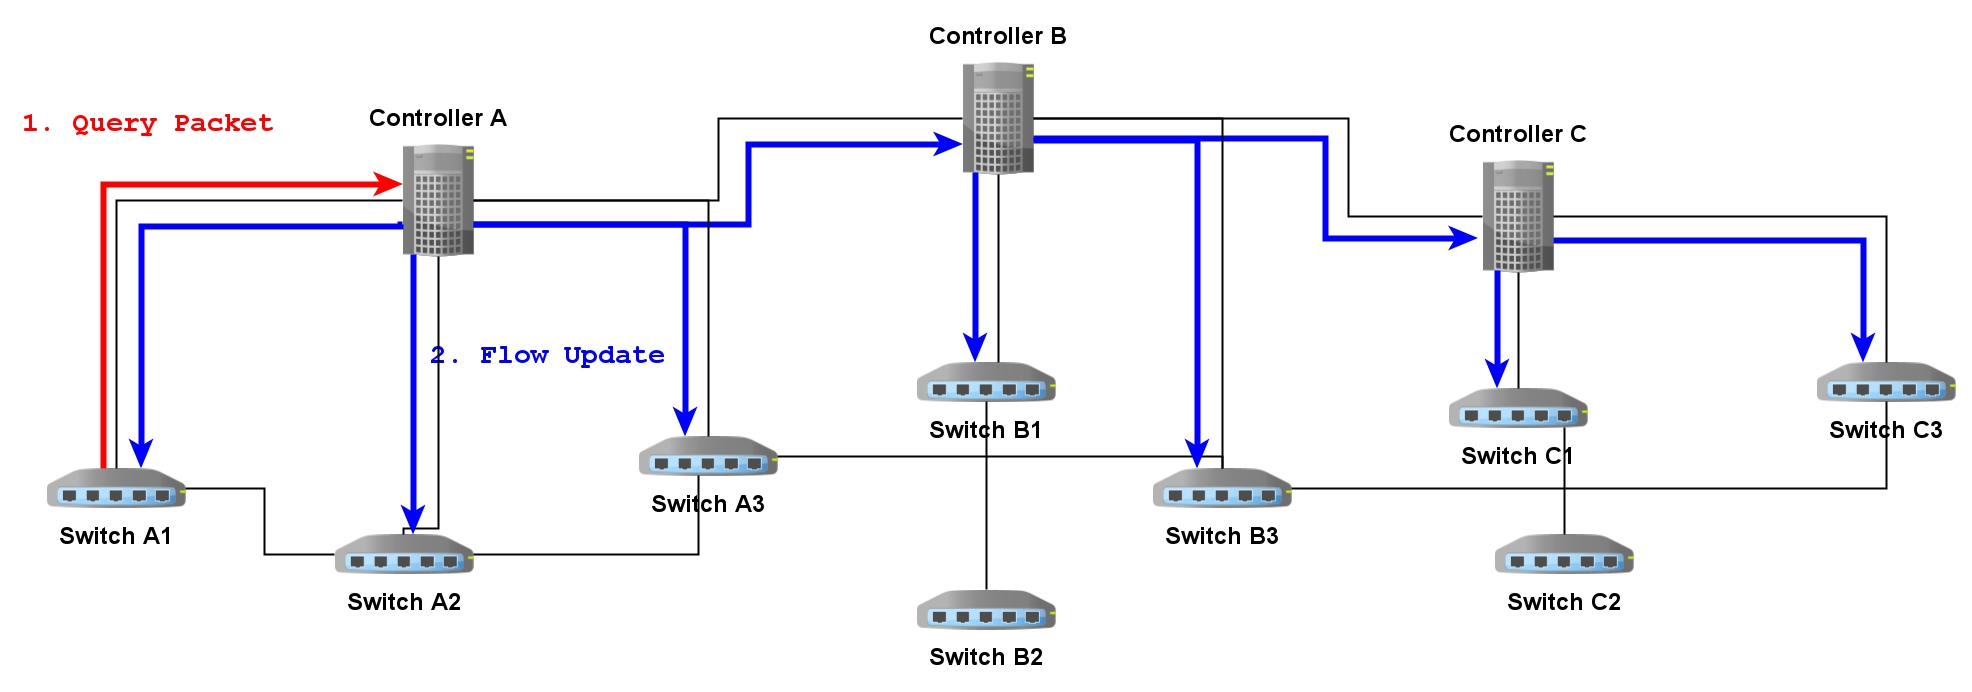
\includegraphics[width=0.45\textwidth]{Images/new_flow.jpg}
		\caption{Setup of a new flow in the flow table} \label{new_flow}
	\end{figure}

	SDN switches match every incoming packet with appropriate flow tables. The result of a match can either be a \textit{hit} - which means the appropriate flow is already in a flow table, or, a \textit{miss} - in which case the flow is new and the switch asks its assigned controller for the next course of action. The assigned controller decides on a path for the flow and notifies the concerned switches to update their flow tables. However, for switches assigned to another controller, the controller is notified instead (Figure \ref{new_flow}). Therefore, the total time required to notify all the concerned switches of the new path is the processing delay of a new flow. I represent the overall flow-setup ($\Omega$) latency of the network as the average notification time of all possible pair of switches in the network. For a network $S$ with $|S|$ number of switches, the flow-setup latency can be calculated as follows:
	
	\begin{equation} \label{eqn:setupLatency}
	\begin{split}
	\Omega(S) = &\frac{2}{|S|\times |S-1|}\sum_{s_i,s_d\in S} \{dis(s_i,c_i)+\\ &\max_{s_j\in path_{i,d}}\left(dis(c_i,c_j)+dis(c_j,s_j) \right) \}
	\end{split}
	\end{equation}
	
	here, $path_{i,d}$ is the shortest path from source $s_i$ to destination $s_d$ and $s_j$ is any switch in that path. The controllers of switches $s_i$ and $s_j$ are $c_i$ and $c_j$ respectively.
	
	\section{Experimental Analysis}
	My proposed mechanism clusters the network, places controllers, and performs load balancing on the clustered network. In the following sections \ref{CPAnalysis} and \ref{optimumK}, I compare our algorithms LBC (with CSA) with renowned controller placement methods and I determine an optimum number of controllers for any given network. In section \ref{LoadAnalysis} I compare my algorithm BLB with state-of-the-art load balancing algorithms \cite{dbcp2017, filali2018sdn}. Simulation results suggest that my proposed mechanism outperforms most advanced algorithms in terms of both overall latency and load balancing.
	
	
	\subsection{Decisive Variables} \label{optimumK}
	LBC clusters the network into $k$ sub-networks and CSA places a controller in each sub-network using the constant $\alpha$, which is a real number ranging from $0$ to $1$. The constant dictates the placement of controllers by controlling the priority of intra-cluster and inter-cluster distances. Applying LBC on a small network with varying values of $k$ and $\alpha$ provide valuable insight on how the two variables affect the overall flow-setup latency of a network (Equation \ref{eqn:setupLatency}).
	
	An increased number of clusters are formed when an excessively large amount of controllers are placed in a network. Consequently, the cluster-sizes are diminished, greatly reducing the number of viable controller positions in a specific cluster. Therefore, for a specific and large value of $k$, varying the value of $\alpha$ causes little or no change in placement and has no effect on overall flow-setup latency (Figure \ref{fig:abileneA}). Taking into consideration the above-mentioned property and observing the values of $\alpha$, I select $0.2$ as the optimum value for the given network. The flow-setup latency of a network decreases as the number of controllers increase, with a few exceptions due to variations in network topology ($k=3$ and $k=2$ in Figure \ref{fig:KvsL}). Accordingly, the setup latency is minimum when $k$ is equal to the total number of nodes in a network, which however, invalidates one of the firsthand benefits of placing controllers (simplifying nodes and reducing costs). In order to establish a cut-off point to minimize both flow-setup latencies and number of controllers, I analyze the latency change in different networks for optimum values of $\alpha$ and varying values of $k$ (Figure \ref{fig:KvsL}).
	
	\begin{figure}
		\centering
		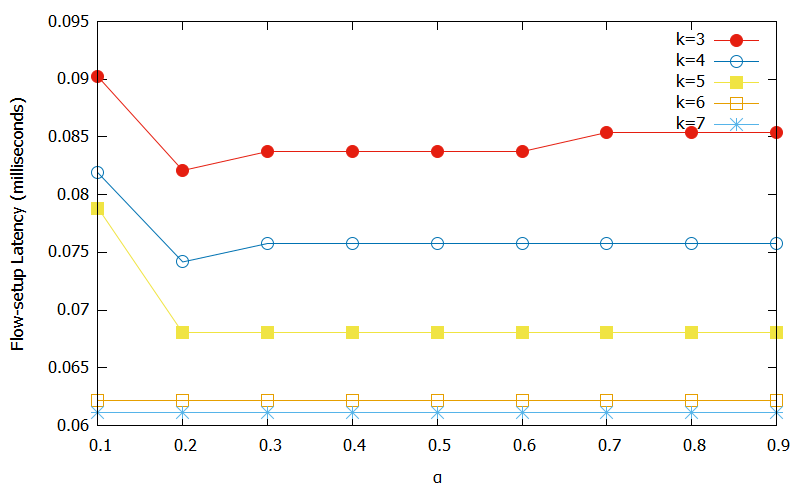
\includegraphics[width=0.45\textwidth]{Images/Abilene_Analysis.png}
		\caption{Flow-setup latencies for varying values of $\alpha$ and $k$} \label{fig:abileneA}
		
		\centering
		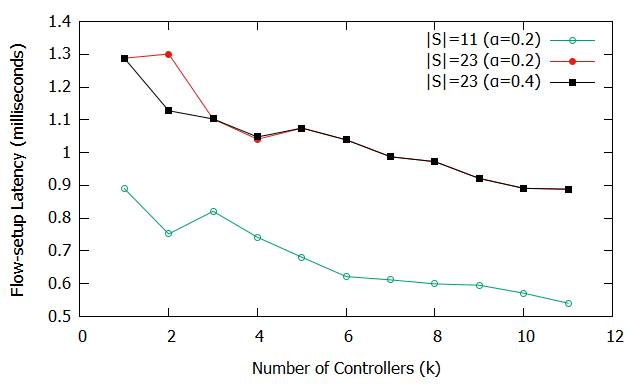
\includegraphics[width=0.45\textwidth]{Images/k_vs_l.png}
		\caption{Decreasing flow-setup latencies with respect to number of controllers ($k$) for different network sizes ($|S|$)} \label{fig:KvsL}
	\end{figure}

	According to \cite{cpp2012heller}, a network with $34$ nodes requires approximately $4$ controllers to function efficiently. Consequently, a controller can operate roughly $8$-$9$ switches  on average with maximized throughput and adequate fault tolerance. Therefore, we derive a utility ratio which calculates the decrease in latency per addition of controller, as follows:
	\begin{equation}
		utility(k) = \frac{Latency(1)}{Latency(k)}
	\end{equation}
	here, $k$ is the number of controllers and $Latency$ refers to flow-setup latency (Equation \ref{eqn:setupLatency}). Comparing the utility ratio with the number of controllers, I determine a cut-off point to calculate the optimum number of controllers for a network (Figure \ref{fig:cutoff}).
	
	\begin{figure}
		\centering
		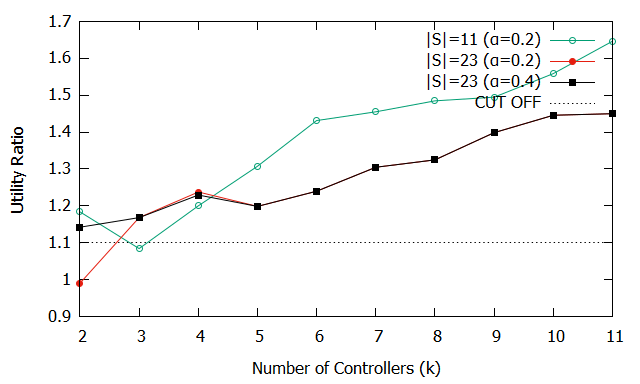
\includegraphics[width=0.45\textwidth]{Images/cutoff.png}
		\caption{Gradually increasing utility ratio with respect to number of controllers ($k$) for different network sizes ($|S|$)} \label{fig:cutoff}
	\end{figure}
	
	\subsection{Controller Placement} \label{CPAnalysis}
	In this section I evaluate my static controller placement method (LBC and CSA) in comparison to the well-known algorithm DBCP and my previous placement algorithm DBC. DBCP places controllers based on the density of nodes and the minimum distance to higher density nodes. In order to compare the algorithms, I simulate both DBC and LBC with the same number of controllers as DBCP when clustering the networks from the Zoo Topology. DBCP underperforms compared to LBC and DBC when the network has high connectivity (e.g. star topology) or when all nodes have equal density (e.g. ring topology). My simulations using the remaining networks suggest that LBC+CSA outperforms both DBCP and DBC in terms of flow-setup latencies. A summary of the several simulations is represented in Table \ref{tab:summ1}.
	
	\begin{table}
		\centering
		\caption{Controller Placement Simulation Summary} \label{tab:summ1}
		\begin{tabular}{|l|c|}
			\hline
			Simulated networks & 238 \\
			\hline
			DBCP outperforms LBC+CSA & 38 \\
			\hline
			DBC outperforms LBC+CSA & 51 \\
			\hline
			LBC+CSA outperforms both & 154 \\
			\hline
		\end{tabular}
	\end{table}
	The flow-setup latency results of the simulations vary greatly for different networks. Therefore, I normalize the latencies of DBCP and DBC as a ratio of the latencies of DBC and compare networks selected at regular intervals (Figure \ref{fig:Fcomparision}). I observe that DBCP performs better for smaller networks and DBC performs better in larger networks. However, LBC+CSA outperforms both DBCP and DBC in terms of normalized flow-setup latencies.
	
	My proposed algorithms LBC and CSA also optimize the number of controllers (see Section \ref{optimumK}) which is demonstrated in Figure \ref{fig:Kcomparison}. According to the LBC simulations, on average the number of controllers ($k$) increase with increasing network size ($|S|$). However, the controllers selected by DBCP vary greatly with network size.

	\begin{figure}
		\centering
		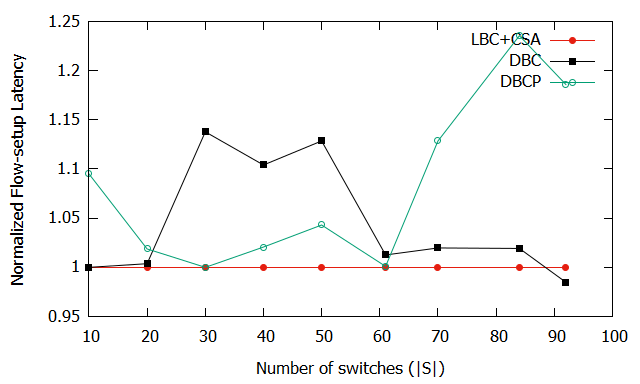
\includegraphics[width=0.45\textwidth]{Images/forced_comparison.png}
		\caption{Comparison among LBC+CSA, DBCP and DBC, in terms of normalized flow-setup latency} \label{fig:Fcomparision}
		\centering
		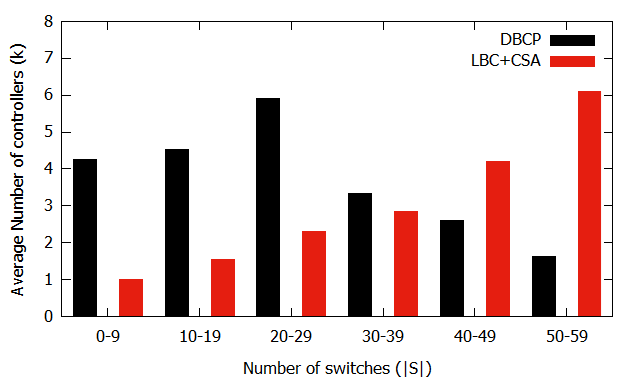
\includegraphics[width=0.45\textwidth]{Images/K.png}
		\caption{Comparison between DBCP and DBC, in terms of average number of controllers} \label{fig:Kcomparison}
	\end{figure}

	\subsection{Load Balancing} \label{LoadAnalysis}
	
	\section{Conclusion}
	
	\bibliographystyle{ieeetran}
	\bibliography{mybib}
\end{document}
